\begin{figure}[t]
    \vspace*{-\figskipabove px}
    \centering
    \hspace*{-22px}
    \begin{subfigure}[t]{0.49\linewidth}
        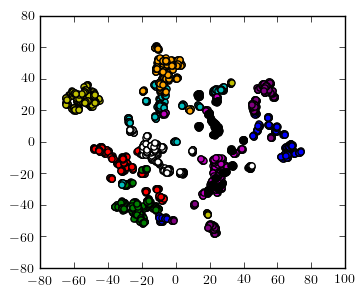
\includegraphics[height=3.1cm]{gls_modelnet10_codes_}
        \subcaption{\bf \DVAE t-SNE}
        \label{fig:results-latent-space-a1}
    \end{subfigure}
    \hspace*{-12px}
    \begin{subfigure}[t]{0.49\linewidth}
        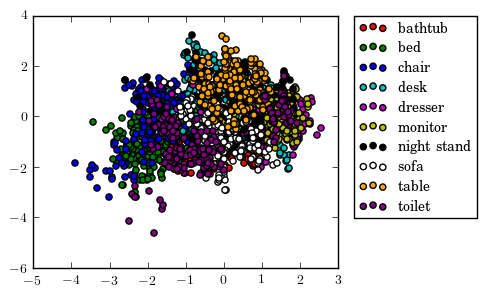
\includegraphics[height=3cm]{gls_modelnet10_codes2}
        \subcaption{\bf \DVAE Projection}
        \label{fig:results-latent-space-a2}
    \end{subfigure}
    \\
    \hspace*{-22px}
    \begin{subfigure}[t]{0.49\linewidth}
        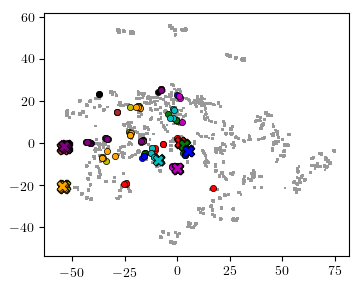
\includegraphics[height=3cm]{gls_clean_codes_outputs_}
        \subcaption{\bf \AML t-SNE}
        \label{fig:results-latent-space-b1}
    \end{subfigure}
    \hspace*{-12px}
    \begin{subfigure}[t]{0.49\linewidth}
        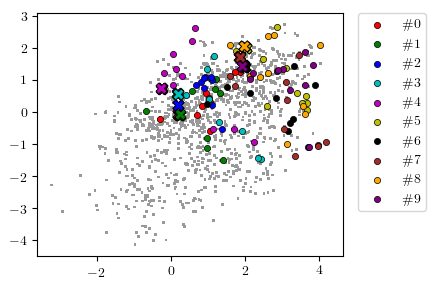
\includegraphics[height=3cm]{gls_clean_codes2_outputs}
        \subcaption{\bf \AML Projection}
        \label{fig:results-latent-space-b2}
    \end{subfigure}
    \vspace*{-\figskipcaption px}
    \caption{{\bf Learned Latent Spaces.} In (\subref{fig:results-latent-space-a1}) and (\subref{fig:results-latent-space-a2}), we show a t-SNE \citep{Maaten2008JMLR} visualization and a two-dimensional projection of the \DVAE latent space on ModelNet10. The plots illustrate that the \DVAE is able to separate the ten object categories. In (\subref{fig:results-latent-space-b1}) and (\subref{fig:results-latent-space-b2}), we show a t-SNE visualization and a projection of the latent space corresponding to our learned \AML model on \clean. We randomly picked $10$ ground truth shapes,  ``x'', and the corresponding observations ($10$ per shape), points (gray pixels indicate remaining shapes/observations). The plots illustrate that \AML is able to associate observations with the corresponding ground truth shapes under weak supervision.}
    \label{fig:results-latent-space}
    \vspace*{-\figskipbelow px}
\end{figure}